\chapter{Moleculaire evolutie en fylogenomica}\label{ch:b3:molecular-evolution}

In 1968 maakte Motoo Kimura een berekening die een vakgebied
verontrustte. Door de hemoglobinen, cytochromen en andere eiwitten te
vergelijken van zoogdieren wier gemeenschappelijke voorouders met
fossielen waren gedateerd, vond hij dat aminozuren waren vervangen met
een tempo van ruwweg één substitutie per plaats per miljard jaar ---
wat, over een genoom van een zoogdier en een generatie, neerkwam op
ongeveer elke twee jaar een nieuwe substitutie die in de populatie werd
vastgelegd. Haldane had een decennium eerder aangetoond dat de
natuurlijke selectie hoogstens ongeveer één substitutie per driehonderd
generaties kan vastleggen voordat de kosten in verloren nakomelingen
onbetaalbaar worden. De rekenkunde liet één uitweg: de meeste
veranderingen die zich in DNA ophopen worden helemaal niet door
selectie gedreven, maar zijn neutraal en worden bij toeval vastgelegd
in eindige populaties, met een tempo dat --- zoals de eerste stelling
van dit hoofdstuk laat zien --- eenvoudigweg het mutatietempo is. De
\omterm{thm:b3:molecular-evolution:neutral}{neutrale theorie} werd de nulhypothese van de moleculaire evolutie, de
maatstaf waartegen selectie wordt opgespoord; de \omterm{prop:b3:molecular-evolution:clock}{moleculaire klok} werd
een manier om te dateren wat fossielen niet konden; en de genomen die
sindsdien zijn bepaald hebben het gereedschap geleverd om gen voor gen
te zien waar de selectie heeft gewerkt, hoe nieuwe genen uit oude
worden geboren, en waarom de boom van een gen niet altijd de boom van
zijn soort is.

\section{Drift, mutatie en het neutrale tempo}

\begin{theorem}[Het neutrale substitutietempo]\label{thm:b3:molecular-evolution:neutral}
\index{neutrale theorie}\index{substitutietempo}\index{fixatiekans}\index{genetische drift}
In een diploïde populatie van $N$ individuen heeft een nieuwe mutatie
zonder gevolgen voor de fitness een kans $1/2N$ om uiteindelijk alle
andere allelen te vervangen (\emph{fixatie}) en een kans $1 - 1/2N$ om
verloren te gaan. Muteert elk van de $2N$ genkopieën met tempo $\mu$
per generatie, dan ontstaan er per generatie $2N\mu$ nieuwe neutrale
mutaties, en is het tempo waarmee substituties zich op den duur ophopen
\[
k = 2N\mu\times\frac{1}{2N} = \mu :
\]
het neutrale \emph{\omterm{thm:b3:molecular-evolution:neutral}{substitutietempo}} is gelijk aan het mutatietempo,
onafhankelijk van de omvang van de populatie. Een mutatie die
voorbestemd is om te worden vastgelegd doet daar gemiddeld $4N$
generaties over, dus houden grote populaties meer variatie onderweg
vast maar leggen zij haar niet sneller vast. Voor een mutatie met een
selectief voordeel $s$ geeft de formule van Kimura de \omterm{thm:b3:molecular-evolution:neutral}{fixatiekans}
\[
P(s) = \frac{1 - \mathrm{e}^{-2s}}{1 - \mathrm{e}^{-4Ns}} \approx 2s
\quad (4Ns \gg 1),
\]
zodat een voordeel van \qty{1}{\%} met een kans van ongeveer
\qty{2}{\%} wordt vastgelegd --- veertig maal de kans van een neutrale
mutatie in een populatie van tweeduizend, maar nog altijd
negenenveertig van de vijftig keer verloren; en een nadeel $s < 0$ met
$4N|s| \gg 1$ wordt vrijwel nooit vastgelegd, terwijl een nadeel met
$4N|s| \ll 1$ zich als neutraal gedraagt: de selectie ziet alleen wat
de drift niet overspoelt, en de grens ligt bij $|s| \sim
1/4N$ --- \emph{effectief neutraal}.
\end{theorem}
\begin{proof}
Neutraliteit: een van de kopieën die er vandaag zijn zal in de verre
toekomst de voorouder van de hele populatie zijn, en uit symmetrie is
elk van de $2N$ kopieën even waarschijnlijk die ene; de nieuwe mutant
is één kopie, vandaar $1/2N$. Tempo: substituties per generatie $=$
(mutaties die per generatie ontstaan) $\times$ (de kans dat elk wordt
vastgelegd) $= 2N\mu/2N$. De formule van Kimura volgt uit de
diffusiebenadering van de verandering van de allelfrequentie onder
drift en selectie, die hier wordt aangenomen; haar limieten worden
rechtstreeks nagegaan: voor $s \to 0$ geldt $(2s)/(4Ns) = 1/2N$, de
neutrale waarde; voor $4Ns \gg 1$ is de noemer $1$ en de teller
$\approx 2s$. Fixatietijd: de frequentie van een neutraal allel voert
een toevalswandeling uit met variantie $p(1-p)/2N$ per generatie, en de
verwachte tijd om $1$ te bereiken vanaf $1/2N$, gegeven dat dat
gebeurt, is $4N$ generaties (Kimura en Ohta, 1969), hier aangenomen.
\end{proof}

\begin{omfigure}
\begin{tikzpicture}
\begin{semilogyaxis}[
  width=0.62\linewidth, height=5.6cm,
  axis x line=bottom, axis y line=left,
  xmin=-4, xmax=8, ymin=0.00002, ymax=0.2,
  xlabel={$4Ns$ (geschaalde selectiecoëfficiënt)}, ylabel={fixatiekans},
  xlabel style={font=\small, at={(axis description cs:0.5,-0.12)}, anchor=north}, ylabel style={font=\small},
  tick label style={font=\small}, xtick={-4,-2,0,2,4,6,8}, ytick={0.0001,0.001,0.01,0.1}, yticklabels={$10^{-4}$,$10^{-3}$,$10^{-2}$,$10^{-1}$},
  clip=false,
]
\addplot[very thick, omDef, domain=-4:-0.05, samples=60] {(x/2000)/(1-exp(-x))};
\addplot[very thick, omDef, domain=0.05:8, samples=80] {(x/2000)/(1-exp(-x))};
\draw[dashed, gray] (axis cs:-4,0.0005) -- (axis cs:8,0.0005); \node[font=\scriptsize, gray, anchor=north west] at (axis cs:-3.9,0.00048) {neutraal, $1/2N$};
\addplot[thick, omThm, dashed, domain=1:8, samples=2] {2*x/(4*1000)};
\node[font=\scriptsize, omThm, anchor=north west] at (axis cs:5,0.0012) {asymptoot $2s$};
\node[font=\scriptsize, omDef, anchor=south east, align=right] at (axis cs:-0.2,0.02) {effectief neutraal\\wanneer $|4Ns| \lesssim 1$};
\node[font=\scriptsize, omDef, anchor=south west] at (axis cs:-3.9,0.0008) {nadelig: vrijwel nooit vastgelegd};
\end{semilogyaxis}
\end{tikzpicture}

{\small De \omterm{thm:b3:molecular-evolution:neutral}{fixatiekans} van Kimura tegen de geschaalde
selectiecoëfficiënt, voor $N = 1000$. Vlak bij nul gaat de kromme door
de neutrale waarde; naar rechts stijgt zij naar $2s$; naar links valt
zij van een klif. De selectie werkt alleen op wat de drift niet kan
verbergen.}
\end{omfigure}

\begin{proof}[Bewijsmateriaal]
Kimura (1968) en King en Jukes (1969) bouwden hun betoog op tempo's:
het waargenomen tempo van aminozuursubstitutie over de eiwitten van
zoogdieren vergde meer substituties per generatie dan de selectiekosten
van Haldane toelieten, dus moesten de meeste neutraal zijn. De
voorspellingen van de theorie hielden vervolgens stand: de tempo's zijn
het hoogst waar de functie het minst beperkt --- synonieme plaatsen,
intronen, \omterm{def:b3:molecular-evolution:duplication}{pseudogenen}, de derde codonpositie --- en het laagst in
\omterm{def:b3:chromatin-epigenetics:nucleosome}{histonen} en ubiquitine, die één residu per honderd miljoen jaar
veranderen; het niveau van variatie binnen een soort volgt het
mutatietempo en de omvang van de populatie; en het tempo van
substitutie per jaar is ruwweg constant over lijnen met zeer
verschillende populatiegroottes, zoals de formule $k = \mu$ vergt en
een selectionistische verklaring niet. De twist die erop volgde heeft
haar niet omvergeworpen: zij heeft het neutrale tempo vastgelegd als de
nulmaat waartegen selectie wordt gemeten.
\end{proof}

\begin{omfigure}
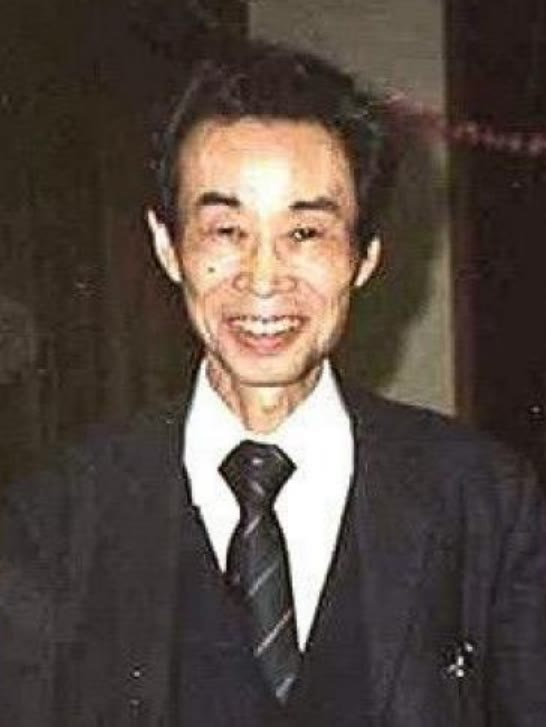
\includegraphics[width=0.34\linewidth]{images/book5/kimura.jpg}\hspace{0.05\linewidth}
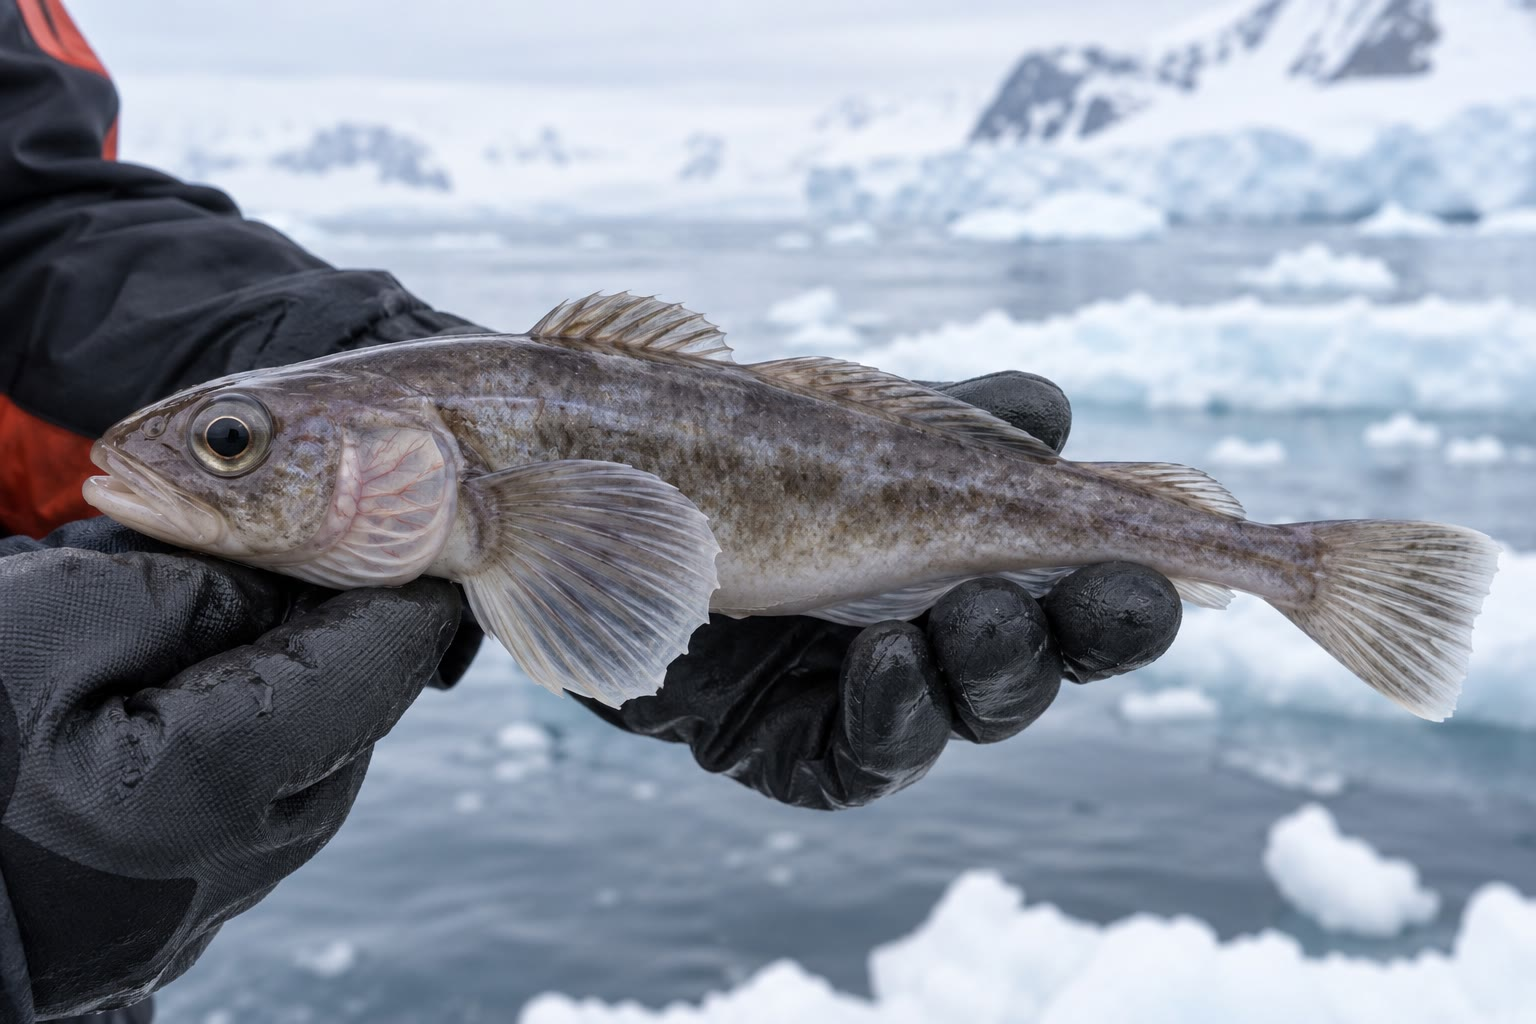
\includegraphics[width=0.5\linewidth]{images/book5/ai/b5-25-icefish.jpg}

{\small Links: Motoo Kimura (1924--1994), die aantoonde dat de meeste
moleculaire verandering bij toeval en met het mutatietempo wordt
vastgelegd (foto, 1986, CC BY 4.0). Rechts: een Antarctische ijsvis,
wier bloed door een antivries-glyco-eiwit uit de vrieskou wordt
gehouden, zo'n tien miljoen jaar geleden samengesteld uit een verdubbeld
gen voor een verteringsenzym en een reeks herhalingen.}
\end{omfigure}

\section{De moleculaire klok}

\begin{proposition}[De klok en haar onregelmatigheden]\label{prop:b3:molecular-evolution:clock}
\index{moleculaire klok}\index{ijking}\index{verschillen in tempo}\index{ontspannen klok}\index{effect van de generatieduur}
Hopen substituties zich met een constant tempo $k$ per plaats per jaar
op in twee lijnen die $T$ jaar geleden zijn gesplitst, dan is het deel
van de plaatsen waarop zij verschillen voor kleine waarden
$d \approx 2kT$: de divergentie van twee sequenties is een
\emph{\omterm{prop:b3:molecular-evolution:clock}{moleculaire klok}} (Zuckerkandl en Pauling, 1965), die met één
door fossielen gedateerde splitsing kan worden \emph{geijkt} en daarna
kan worden afgelezen voor splitsingen zonder fossielen. De klok is
stochastisch --- een Poisson-proces, dus heeft $d$ over een vast aantal
plaatsen een variantie die ongeveer gelijk is aan haar gemiddelde ---
en zij is op drie bekende manieren onregelmatig. Elk eiwit heeft zijn
eigen tempo, bepaald door het deel van zijn plaatsen dat de functie
laat veranderen: fibrinopeptiden \num{8}, hemoglobine \num{1},
cytochroom~$c$ \num{0.3}, \omterm{def:b3:chromatin-epigenetics:nucleosome}{histon}~H4 \num{0.01} substituties per plaats
per miljard jaar. De tempo's verschillen tussen lijnen: omdat het
neutrale tempo $\mu$ per generatie is, hopen dieren met korte
generaties (knaagdieren) per jaar meer verandering op dan dieren met
lange (primaten, walvissen) --- het \emph{\omterm{prop:b3:molecular-evolution:clock}{effect van de generatieduur}},
dat ten dele wordt opgeheven doordat het mutatietempo per generatie met
de generatieduur stijgt. En $d$ verzadigt: zodra er veel plaatsen zijn
veranderd, treffen verdere veranderingen plaatsen die al zijn
veranderd, zodat het ruwe verschil voor meervoudige treffers moet
worden gecorrigeerd, zoals de afstanden van het hoofdstuk over
\omterm{def:b3:bioinformatics:alignment}{uitlijning} doen. Moderne \emph{ontspannen klokken} laten het tempo
binnen een statistisch model tussen takken variëren en worden met vele
fossielen tegelijk geijkt; zij dateren de splitsing van mens en
chimpansee op zes tot zeven miljoen jaar, die van de ordes van de
placentadieren nabij het einde van het Krijt, en die van dieren en
schimmels in het Precambrium, met onzekerheden van tien tot twintig
procent die vooral van de fossielen komen.
\end{proposition}
\begin{proof}
Elke lijn hoopt $kT$ substituties per plaats op, dus is het verschil
ertussen $2kT$ waar plaatsen niet tweemaal zijn getroffen; een paar dat
met fossielen is gedateerd geeft $k = d/2T$. De Poisson-variantie en de
tempo's per eiwit zijn die van Zuckerkandl en Pauling, van Dickerson
(1971) en van de fits van Kimura aan verzamelingen eiwitten van
gewervelden; de verzadigingscorrectie is de formule van Jukes en Cantor
uit het hoofdstuk over \omterm{def:b3:bioinformatics:alignment}{uitlijning}, $d_{\text{true}} =
-\tfrac{3}{4}\ln(1 - \tfrac{4}{3}p)$. \omterm{prop:b3:molecular-evolution:clock}{Verschillen in tempo} tussen
lijnen werden aangetoond met toetsen op het relatieve tempo: met een
buitengroep $O$ en twee soorten $A$ en $B$ zou $d_{AO} - d_{BO}$ onder
een strenge klok nul moeten zijn, en dat is het niet voor knaagdieren
tegen primaten.
\end{proof}

\begin{omfigure}
\begin{tikzpicture}
\begin{axis}[
  width=0.68\linewidth, height=5.8cm,
  axis x line=bottom, axis y line=left,
  xmin=0, xmax=600, ymin=0, ymax=110,
  xlabel={tijd sinds de divergentie (miljoen jaar)}, ylabel={substituties per 100 plaatsen (gecorrigeerd)},
  xlabel style={font=\small, at={(axis description cs:0.5,-0.12)}, anchor=north}, ylabel style={font=\small},
  tick label style={font=\small}, xtick={0,100,200,300,400,500,600}, ytick={0,20,40,60,80,100},
  clip=false,
]
\addplot[very thick, omThm, domain=0:130, samples=2] {2*0.4*x};
\addplot[very thick, omDef, domain=0:600, samples=2] {2*0.09*x};
\addplot[very thick, omMeth!70!black, domain=0:600, samples=2] {2*0.03*x};
\addplot[very thick, omProp!80!black, domain=0:600, samples=2] {2*0.001*x};
\addplot[only marks, mark=*, mark size=1.8pt, omDef] coordinates {(80,13) (100,20) (300,52) (400,75) (450,80)};
\addplot[only marks, mark=*, mark size=1.8pt, omMeth!70!black] coordinates {(80,4) (300,17) (450,29) (550,33)};
\addplot[only marks, mark=*, mark size=1.8pt, omThm] coordinates {(30,22) (80,68) (100,80)};
\node[font=\scriptsize, omThm, anchor=west] at (axis cs:132,104) {fibrinopeptiden};
\node[font=\scriptsize, omDef, anchor=south east] at (axis cs:600,108) {hemoglobine};
\node[font=\scriptsize, omMeth!70!black, anchor=north west] at (axis cs:530,35) {cytochroom $c$};
\node[font=\scriptsize, omProp!80!black, anchor=south east] at (axis cs:600,1.5) {histon H4};
\end{axis}
\end{tikzpicture}

{\small De \omterm{prop:b3:molecular-evolution:clock}{moleculaire klok}, eiwit voor eiwit. Elk loopt met zijn eigen
tempo, bepaald door hoeveel van het molecuul de functie vrij laat om te
veranderen: een fibrinopeptide, dat bij het stollen van bloed wordt
afgeknipt en weggegooid, verandert honderden malen sneller dan het
\omterm{def:b3:chromatin-epigenetics:nucleosome}{histon} dat DNA inpakt.}
\end{omfigure}

\section{Selectie aflezen in sequenties}

\begin{definition}[dN/dS]\label{def:b3:molecular-evolution:dnds}
\index{synonieme substitutie}\index{niet-synonieme substitutie}\index{dN/dS-verhouding}\index{zuiverende selectie}\index{positieve selectie}
In een eiwitcoderend gen is een substitutie \emph{synoniem} wanneer zij
het aminozuur onveranderd laat en \emph{niet-synoniem} wanneer zij het
verandert. Omdat de genetische code de meeste derde posities en sommige
eerste posities stilzwijgend laat veranderen, is ongeveer een kwart van
de mogelijke mutaties in een gewoon gen synoniem. Zij $d_{S}$ het
aantal synonieme substituties per synonieme plaats en $d_{N}$ het
aantal niet-synonieme substituties per niet-synonieme plaats, beide
gecorrigeerd voor meervoudige treffers. Synonieme veranderingen liggen
dicht bij neutraal, dus schat $d_{S}$ de waarde $2\mu T$ --- de klok;
en de verhouding
\[
\omega = \frac{d_{N}}{d_{S}}
\]
meet wat de selectie met het eiwit heeft gedaan: $\omega = 1$ als
veranderingen van aminozuren even vrij zijn als stille veranderingen
(geen beperking, zoals in een \omterm{def:b3:molecular-evolution:duplication}{pseudogen}); $\omega < 1$ onder
\emph{zuiverende selectie}, waarbij de meeste veranderingen worden
verwijderd --- het gewone gen heeft $\omega \approx 0.1$ tot $0.2$,
\omterm{def:b3:chromatin-epigenetics:nucleosome}{histonen} $0.001$; $\omega > 1$ onder \emph{positieve selectie}, waarbij
veranderingen van aminozuren sneller worden begunstigd dan de drift
alleen toelaat --- de antigeenbindende groeve van MHC-moleculen, de
oppervlakte-eiwitten van virussen in een wapenwedloop met antilichamen,
de eiwitten van zaadcel en eicel bij de bevruchting, en het lysozym van
herkauwers, dat is ingelijfd om bacteriën in de maag te verteren.
Berekend langs één tak van een boom of plaats voor plaats brengt
$\omega$ in kaart waar en wanneer een eiwit door selectie en niet door
toeval is veranderd.
\end{definition}

\begin{omfigure}
\begin{tikzpicture}[every node/.style={font=\scriptsize}, >=stealth]
  \begin{axis}[
    width=0.52\linewidth, height=5.2cm,
    xbar, bar width=7pt, y=0.45cm,
    axis x line=bottom, axis y line=left,
    xmin=0.0005, xmax=5, xmode=log,
    xlabel={$\omega = d_{N}/d_{S}$},
    xlabel style={font=\small, at={(axis description cs:0.5,-0.12)}, anchor=north},
    symbolic y coords={histon H4, actine, insuline, gewoon gen, cytochroom $c$, pseudogen, lysozym herkauwer, MHC-groeve, hiv-envelop},
    ytick=data, tick label style={font=\scriptsize},
    xtick={0.001,0.01,0.1,1}, xticklabels={0.001,0.01,0.1,1},
    clip=false,
  ]
  \addplot[fill=omDef!50, draw=omDef] coordinates {(0.002,histon H4) (0.01,actine) (0.09,insuline) (0.15,gewoon gen) (0.05,cytochroom $c$) (1,pseudogen) (2.5,lysozym herkauwer) (3.5,MHC-groeve) (4,hiv-envelop)};
  \draw[dashed, thick, omThm] (axis cs:1,histon H4) -- (axis cs:1,hiv-envelop);
  \node[omThm, anchor=south, font=\tiny] at (axis cs:1,hiv-envelop) {$\omega = 1$: neutraal};
  \node[anchor=east, font=\tiny, gray] at (axis cs:0.5,actine) {zuiverend};
  \node[anchor=west, font=\tiny, gray] at (axis cs:1.6,insuline) {positief};
  \end{axis}
\end{tikzpicture}

{\small Ordes van grootte van $\omega$. Vrijwel elk gen ligt ver onder
één, met zijn aminozuren bewaakt door \omterm{def:b3:molecular-evolution:dnds}{zuiverende selectie}; een
\omterm{def:b3:molecular-evolution:duplication}{pseudogen} drijft bij één; de weinige boven één zijn de eiwitten in
wapenwedlopen of die pas voor een nieuwe taak zijn ingelijfd.}
\end{omfigure}

\begin{method}[$d_{N}/d_{S}$ schatten]\label{met:b3:molecular-evolution:method}
\index{codonuitlijning}
(1) Lijn de twee coderende sequenties codon voor codon uit (lijn de
eiwitten uit en breng ze daarna terug op het DNA, zodat geen gat het
leesraam breekt). (2) Tel voor elk codon de synonieme en niet-synonieme
\emph{plaatsen}: elk van de drie posities wordt gescoord met het deel
van de mogelijke veranderingen dat stil is --- een viervoudig
gedegenereerde derde positie telt als één synonieme plaats, een positie
waar elke verandering het aminozuur wijzigt als één niet-synonieme
plaats, een tweevoudige positie als een derde van de ene en twee derde
van de andere. Sommeer over de codons: $S$ synonieme en $N$
niet-synonieme plaatsen, met $S + N = 3 \times$ het aantal codons.
(3) Tel de synonieme en niet-synonieme \emph{verschillen} tussen de
sequenties, en los codons die op twee posities verschillen op door over
de mogelijke paden te middelen. (4) $p_{S} = $ verschillen$/S$,
$p_{N} = $ verschillen$/N$; corrigeer elk voor meervoudige treffers met
Jukes--Cantor. (5) $\omega =
d_{N}/d_{S}$; toets $\omega \ne 1$ tegen de steekproefvariantie, die
groot is wanneer $d_{S}$ klein is --- twee nauw verwante sequenties
geven een onbetrouwbare verhouding, en twee zeer verre hebben een
verzadigde $d_{S}$. (6) Voor waar en wanneer: fit $\omega$ per tak van
een boom, of per plaats met een mengsel van plaatsklassen, en toets of
een klasse met $\omega > 1$ de fit verbetert.
\end{method}

\section{Nieuwe genen uit oude}

\begin{definition}[Verdubbeling, families en overdracht]\label{def:b3:molecular-evolution:duplication}
\index{genverdubbeling}\index{genfamilie}\index{neofunctionalisatie}\index{subfunctionalisatie}\index{pseudogen}\index{horizontale genoverdracht}
De meeste nieuwe genen zijn kopieën van oude. Een
\emph{genverdubbeling} --- door ongelijke overkruising, door
retrotranspositie, of door de verdubbeling van een heel genoom, zoals
tweemaal gebeurde bij de oorsprong van de gewervelden en opnieuw bij de
voorouder van de beenvissen en in vele plantenlijnen --- laat twee
paralogen waar er één was; genen in verschillende soorten die
van één voorouderlijk gen afstammen heten \omterm{def:b3:genomics:comparative}{orthologen}. Het gewone
lot van de kopie is verval: bevrijd van beperking ($\omega \to 1$)
verzamelt zij een stopcodon of een leesraamverschuiving en wordt zij
een \emph{pseudogen}, waarvan het menselijke genoom er zo'n
twintigduizend draagt. Soms overleven beide: door
\emph{neofunctionalisatie}, waarbij de ene kopie een nieuwe functie
verwerft terwijl de andere de oude behoudt (het antivries-glyco-eiwit
van de ijsvis, uit een gen voor trypsinogeen; de rode en groene
opsinen van de primaten, uit een verdubbeling van veertig miljoen jaar
geleden die het trichromatische zien gaf dat het deel van het eerste
jaar beschreef; de kristallinen van de ooglens, uit
stofwisselingsenzymen); of door \emph{subfunctionalisatie}, waarbij
elke kopie een deel van de expressie of de werking van de voorouder
behoudt zodat beide nodig zijn. Herhaalde verdubbeling bouwt
\emph{genfamilies} --- de globinen, de Hox-clusters van het hoofdstuk
over de ontwikkeling, de duizend genen voor \omterm{def:b3:sensory-systems:chemical}{reukreceptoren} van een
muis, waarvan er bij de mens een derde pseudogen is. De andere bron van
nieuwe genen is de \emph{horizontale overdracht}: bacteriën verwerven
genen van niet-verwante bacteriën via \omterm{def:b3:genetic-engineering:tools}{plasmiden}, fagen en vrij DNA, en
zo steekt \omterm{def:b3:bacteriology:resistance}{resistentie tegen antibiotica} in een ziekenhuis de soortgrens
over en is de ``soort'' van een bacterie een kerngenoom omringd door
een verschuivende wolk; bij eukaryoten is overdracht zeldzamer maar wel
degelijk aanwezig --- het \omterm{def:b3:genetic-engineering:plants}{T-DNA} dat \emph{\omterm{def:b3:genetic-engineering:plants}{Agrobacterium}} in planten
invoegt, bacteriegenen in raderdiertjes, en de oeroude massale
overdrachten die de mitochondrie en de chloroplast waren. Waar
overdracht gewoon is, is de geschiedenis van het leven een netwerk, en
is de boom die uit één gen wordt getekend de boom van dat gen.
\end{definition}

\begin{omfigure}
\begin{tikzpicture}[every node/.style={font=\scriptsize}, >=stealth]
  \node[draw, thick, rounded corners, fill=omDef!25, minimum width=1.8cm] (a) at (0,3) {voorouderlijk gen};
  \node[draw, thick, rounded corners, fill=omDef!25, minimum width=1.2cm] (c1) at (-1.2,1.6) {kopie 1};
  \node[draw, thick, rounded corners, fill=omDef!25, minimum width=1.2cm] (c2) at (1.2,1.6) {kopie 2};
  \draw[->, thick] (a) -- (c1); \draw[->, thick] (a) -- (c2); \node[right, font=\tiny] at (0.9,2.4) {verdubbeling};
  \node[draw, thick, rounded corners, fill=gray!20, align=center] (ps) at (-3.6,-0.2) {pseudogen\\$\omega \to 1$, dan\\stopcodons, verval};
  \node[draw, thick, rounded corners, fill=omThm!20, align=center] (neo) at (0,-0.2) {neofunctionalisatie\\één kopie neemt een nieuwe taak\\(antivries, rood/groen opsine)};
  \node[draw, thick, rounded corners, fill=omMeth!25, align=center] (sub) at (3.9,-0.2) {subfunctionalisatie\\elke kopie behoudt een deel\\van de oude expressie};
  \draw[->, thick] (c1.south) -- (ps.north); \draw[->, thick] (c2.south) -- (neo.north); \draw[->, thick] (c2.south) -- (sub.north);
  \node[right, align=left, font=\tiny] at (5.9,1.6) {gewoonste lot: verlies binnen\\enkele miljoenen jaren ($\sim$\num{20000}\\pseudogenen in het menselijke genoom)};
  \node[right, align=left, font=\tiny] at (5.9,0.4) {zeldzamer: beide behouden, en een\\genfamilie groeit (globinen, Hox,\\\num{1000} reukreceptoren)};
  \node[right, align=left, font=\tiny] at (5.9,-0.8) {horizontale overdracht: een gen\\komt van een andere soort ---\\gewoon bij bacteriën};
\end{tikzpicture}

{\small De lotgevallen van een verdubbeld gen. Bevrijd van beperking
vervalt de extra kopie gewoonlijk; nu en dan wordt zij door selectie
voor een nieuwe functie opgevangen, of verdelen de twee kopieën de oude
onder elkaar.}
\end{omfigure}

\begin{proof}[Bewijsmateriaal]
Ohno (1970) stelde verdubbeling voor als de belangrijkste bron van
nieuwe genen voordat er ook maar één familie was gesequenced; de
globinen bevestigden het, met een boom van $\alpha$, $\beta$,
$\gamma$, $\delta$, myoglobine en de globinen van planten en bacteriën
die de data van de verdubbelingen liet samenvallen met de straling van
de gewervelden. Chen, DeVries en Cheng (1997) toonden aan dat het
antivriesgen van de ijsvis zijn signaalsequentie en zijn flankerende
sequenties met trypsinogeen deelt en dat de antivriesherhalingen zijn
ontstaan door de uitbreiding van een stukje van negen nucleotiden dat
een grens tussen intron en exon overspant: een nieuw eiwit uit de losse
onderdelen van een verteringsenzym, door de klok gedateerd op het
bevriezen van de Zuidelijke Oceaan. Thornton en collega's (2006)
reconstrueerden de voorouderlijke sequentie van de steroïdreceptoren,
maakten het eiwit van 450 miljoen jaar oud na, en vonden dat het alleen
op oestrogenen antwoordde; twee latere substituties, die zij aanwezen
en toetsten, verlegden de voorkeur van de verdubbelde kopie naar
cortisol --- een herrezen voorouder, en de weg tussen hem en zijn
nakomelingen in het laboratorium afgelegd.
\end{proof}

\section{Genbomen en soortbomen}

\begin{proposition}[Onvolledige sortering van lijnen]\label{prop:b3:molecular-evolution:ils}
\index{genboom}\index{soortboom}\index{onvolledige sortering van lijnen}\index{coalescent}\index{fylogenomica}
De boom van een gen hoeft niet overeen te komen met de boom van de
soorten die het dragen. Neem drie soorten met \omterm{prop:b3:molecular-evolution:ils}{soortboom} $((A,B),C)$,
waarbij de splitsing van $A$ en $B$ werd voorafgegaan door een
voorouderlijke populatie van omvang $N$ die $T$ generaties bleef
bestaan vóór de splitsing van $C$. Twee genkopieën, één uit $A$ en één
uit $B$, \emph{versmelten} teruggevolgd in een gemeenschappelijke
voorouder met een tempo $1/2N$ per generatie; de kans dat zij nog niet
zijn versmolten wanneer zij de populatie binnengaan die voorouder van
alle drie is, bedraagt $\mathrm{e}^{-T/2N}$, en daarna versmelten de
drie lijnen in willekeurige volgorde, zodat de \omterm{prop:b3:molecular-evolution:ils}{genboom} twee derde van
de keren $A$ of $B$ met $C$ groepeert. De kans dat de \omterm{prop:b3:molecular-evolution:ils}{genboom} met de
\omterm{prop:b3:molecular-evolution:ils}{soortboom} in strijd is bedraagt dus
\[
P_{\text{discord}} = \tfrac{2}{3}\,\mathrm{e}^{-T/2N} .
\]
Voor mens, chimpansee en gorilla, met $T$ van enkele honderdduizenden
generaties en $N$ nabij \num{50000}, steunt ongeveer een derde van het
genoom een boom waarin de mens dichter bij de gorilla staat of de
chimpansee dichter bij de gorilla dan de \omterm{prop:b3:molecular-evolution:ils}{soortboom} zegt --- en dat
wordt waargenomen. Deze \emph{\omterm{prop:b3:molecular-evolution:ils}{onvolledige sortering van lijnen}} is,
samen met verdubbeling en verlies en horizontale overdracht, de reden
dat de \emph{fylogenomica} de \omterm{prop:b3:molecular-evolution:ils}{soortboom} afleidt uit duizenden \omterm{prop:b3:molecular-evolution:ils}{genbomen}
onder een model van de coalescent, en niet door ze aaneen te schakelen
en er één te tekenen; zij laat ook toe de voorouderlijke
populatiegroottes zelf te schatten uit het deel van de bomen dat
afwijkt, en oude kruisingen (neanderthaler-DNA in de moderne mens, de
genstroom tussen beren en tussen vlinders) af te lezen uit bomen die in
een richting afwijken die drift alleen niet zou voortbrengen.
\end{proposition}
\begin{proof}
Twee lijnen in een diploïde populatie van $N$ kiezen elke generatie
ouders uit $2N$ kopieën en delen er met kans $1/2N$ een; over $T$
generaties is de kans dat zij dat nooit doen $(1 - 1/2N)^{T} \approx
\mathrm{e}^{-T/2N}$. Drie lijnen die de gemeenschappelijke
voorouderlijke populatie binnengaan zijn onderling verwisselbaar, dus
is het eerste paar dat versmelt elk van de drie paren met kans $1/3$;
alleen het paar $(A,B)$ komt met de \omterm{prop:b3:molecular-evolution:ils}{soortboom} overeen, dus is $2/3$ van
deze gevallen strijdig. Noch het tempo van de coalescent noch de
verwisselbaarheid hangt van het gen af, dus geldt de formule
onafhankelijk voor elke neutrale locus, en schat het deel strijdige
bomen over een genoom $\mathrm{e}^{-T/2N}$.
\end{proof}

\begin{omfigure}
\begin{tikzpicture}[every node/.style={font=\scriptsize}, >=stealth]
  % species tree as thick grey tubes
  \fill[gray!25] (0,0) -- (0.9,0) -- (2.8,4.2) -- (1.9,4.2) -- cycle;
  \fill[gray!25] (1.6,0) -- (2.5,0) -- (2.8,4.2) -- (1.9,4.2) -- cycle;
  \fill[gray!25] (2.35,2.6) -- (3.15,2.6) -- (3.15,0) -- (3.9,0) -- (3.9,3.4) -- (3.2,5.6) -- (2.3,5.6) -- (1.9,4.2) -- (2.8,4.2) -- cycle;
  \node[below] at (0.45,0) {A}; \node[below] at (2.05,0) {B}; \node[below] at (3.5,0) {C};
  \node[above left, font=\tiny, gray!70!black] at (1.0,4.2) {splitsing A--B};
  \node[above left, font=\tiny, gray!70!black] at (1.0,5.6) {splitsing van C};
  \draw[<->, gray!70!black] (-0.2,4.2) -- (-0.2,5.6) node[midway, left, font=\tiny, align=right] {$T$ generaties,\\omvang $N$};
  \draw[gray!50, dashed] (-0.2,4.2) -- (1.9,4.2); \draw[gray!50, dashed] (-0.2,5.6) -- (2.3,5.6);
  % concordant gene lineages (blue)
  \draw[very thick, omDef] (0.4,0) -- (2.1,3.8) -- (2.2,4.0); \draw[very thick, omDef] (2.0,0) -- (2.2,4.0); \draw[very thick, omDef] (2.2,4.0) -- (2.6,5.0); \draw[very thick, omDef] (3.5,0) -- (2.6,5.0);
  \node[right, align=left, omDef] at (4.6,4.6) {blauw: A en B versmelten vóór\\de splitsing van C --- overeenstemmend};
  % discordant lineages (red)
  \draw[very thick, omThm, dashed] (0.55,0) -- (2.35,4.2) -- (2.7,5.9); \draw[very thick, omThm, dashed] (2.15,0) -- (2.55,4.2) -- (2.9,5.3) -- (3.0,5.5); \draw[very thick, omThm, dashed] (3.65,0) -- (3.0,5.5); \draw[very thick, omThm, dashed] (3.0,5.5) -- (2.7,5.9);
  \node[right, align=left, omThm] at (4.6,3.2) {rood: zij versmelten niet in de\\voorouderlijke populatie (kans\\$\mathrm{e}^{-T/2N}$), en B voegt zich dan eerst bij C:\\de genboom is $((B,C),A)$};
  \node[right, align=left] at (4.6,1.4) {$P_{\text{discord}} = \tfrac{2}{3}\,\mathrm{e}^{-T/2N}$:\\bij $T = 2N$ wijkt één op de vier genen\\van de soortboom af};
\end{tikzpicture}

{\small \omterm{prop:b3:molecular-evolution:ils}{Genbomen} binnen een \omterm{prop:b3:molecular-evolution:ils}{soortboom}. De grijze buizen zijn
populaties; de lijnen zijn de afstamming van één gen. Lijnen die elkaar
in de korte voorouderlijke populatie niet ontmoeten gaan samen de
diepere binnen en paren daar willekeurig af --- zodat een derde van het
genoom van drie dicht opeenvolgende soorten een ander verhaal vertelt
dan de soorten zelf.}
\end{omfigure}

\begin{example}[De geschiedenis van een genoom lezen]\label{ex:b3:molecular-evolution:cichlids}
De vijfhonderd cichlidesoorten van het Victoriameer zijn ontstaan in de
vijftienduizend jaar sinds het meer zich opnieuw vulde --- te snel voor
mutatie om de verschillen ertussen te leveren. Hun genomen laten zien
hoe: de varianten die een bodemeter van een algenschraper onderscheiden
waren al als staande variatie aanwezig in de riviervissen die het meer
koloniseerden, gesorteerd en opnieuw gecombineerd, en aangevuld door
kruising tussen lijnen; de opsinegenen werden op helder of troebel
water afgestemd door substituties waarvan de $\omega$ van hun takken
laat zien dat zij zijn geselecteerd; en de \omterm{prop:b3:molecular-evolution:ils}{genbomen} wijken over het
genoom van elkaar af in precies het patroon dat \omterm{prop:b3:molecular-evolution:ils}{onvolledige sortering
van lijnen} en genstroom voorspellen. Een straling is niet het ontstaan
van nieuwe genen maar het herverdelen van oude allelen over nieuwe
combinaties onder nieuwe selectie --- en de sequenties leggen dat allel
voor allel vast, als men een boom kan lezen die in werkelijkheid een
bos is.
\end{example}

\begin{omfigure}
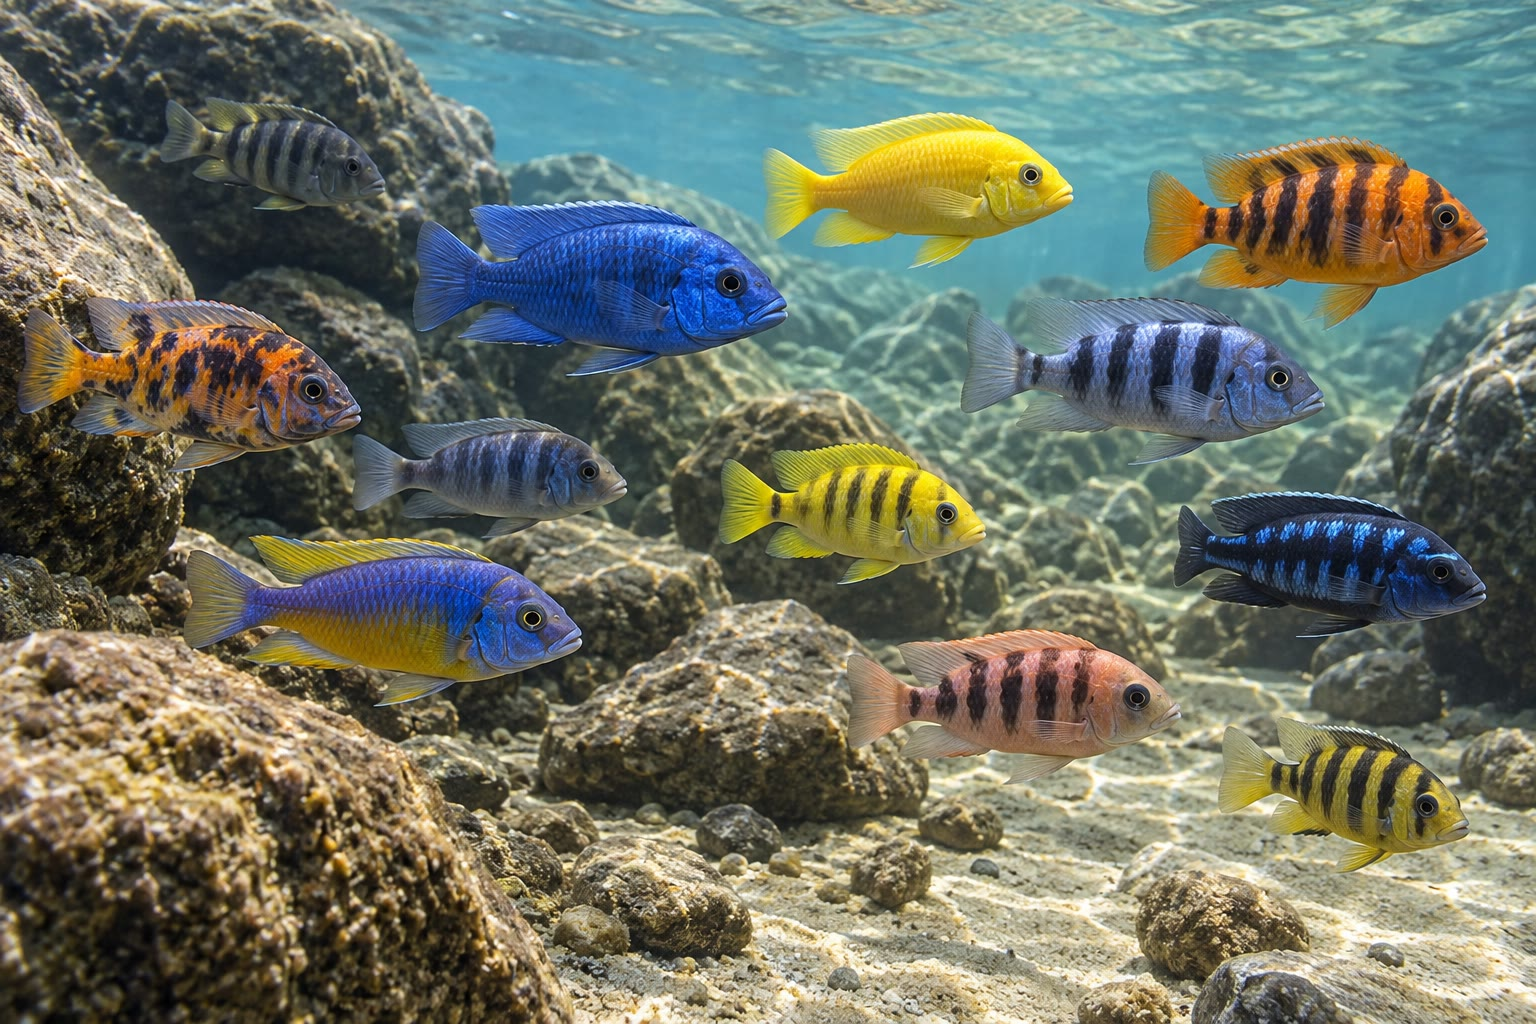
\includegraphics[width=0.6\linewidth]{images/book5/ai/b5-25-cichlids.jpg}

{\small Cichliden van een Afrikaans meer: honderden soorten in een paar
duizend jaar, met verschillen die grotendeels zijn geput uit variatie
die hun gemeenschappelijke voorouders al droegen.}
\end{omfigure}

\begin{remark}[Het toeval als maatstaf]\label{rem:b3:molecular-evolution:remark}
De \omterm{thm:b3:molecular-evolution:neutral}{neutrale theorie} beweert niet dat selectie onbelangrijk is; zij zegt
wat er gebeurt wanneer selectie ontbreekt, nauwkeurig genoeg om
ertegen te worden getoetst. Omdat het neutrale tempo het mutatietempo
is, meet de divergentie de tijd; omdat neutrale verandering de plaatsen
vult die de selectie vrijlaat, meet $\omega$ de beperking; omdat
neutrale lijnen met een bekend tempo versmelten, meet de onenigheid van
\omterm{prop:b3:molecular-evolution:ils}{genbomen} de omvang van populaties die niemand heeft gezien. Selectie is
dan wat er overblijft nadat het toeval is afgetrokken --- een gen met
een $\omega$ boven één, een sweep die de variatie uit een gebied heeft
geveegd, een boom die afwijkt in een richting die drift niet kan
verklaren. Het antivries van de Antarctische ijsvis, het maaglysozym
van de herkauwer en het derde opsine van de primaat zijn de
uitzonderingen die zo zijn gevonden, en elk is een verhaal van een
gekopieerd gen en een nieuwe taak. De rest van het genoom is een klok.
\end{remark}

\section{Opgaven}

\begin{exercise}[$\star$]\label{exo:b3:molecular-evolution:1}
Formuleer het neutrale \omterm{thm:b3:molecular-evolution:neutral}{substitutietempo} en leg in woorden uit waarom
het niet van de omvang van de populatie afhangt.
\end{exercise}

\begin{exercise}[$\star$]\label{exo:b3:molecular-evolution:2}
Definieer \omterm{def:b3:genomics:comparative}{ortholoog}, \omterm{def:b3:genomics:comparative}{paraloog} en \omterm{def:b3:molecular-evolution:duplication}{pseudogen}, met van elk één voorbeeld
uit de globinefamilie.
\end{exercise}

\begin{exercise}[$\star$]\label{exo:b3:molecular-evolution:3}
Wat meet $\omega = d_{N}/d_{S}$? Duid $\omega = 0.02$, $\omega = 1.0$
en $\omega = 2.5$, en noem van elke soort een gen.
\end{exercise}

\begin{exercise}[$\star$]\label{exo:b3:molecular-evolution:4}
Waarom besloot Kimura dat de meeste substituties neutraal zijn? Geef
het betoog opnieuw met de getallen uit de opening van dit hoofdstuk.
\end{exercise}

\begin{exercise}[$\star\star$]\label{exo:b3:molecular-evolution:5}
$N = 5000$. Bereken met de formule van Kimura de \omterm{thm:b3:molecular-evolution:neutral}{fixatiekans} van een
nieuwe mutatie met $s
= 0$, $s = 0.001$, $s = 0.01$ en $s = -0.001$, en geef commentaar op
welke daarvan effectief neutraal zijn.
\end{exercise}

\begin{exercise}[$\star\star$]\label{exo:b3:molecular-evolution:6}
Twee soorten verschillen op \qty{12}{\%} van de plaatsen van een gen
waarvan het neutrale tempo \qty{2e-9}{} per plaats per jaar is. Schat
hun divergentietijd met en zonder de correctie van Jukes en Cantor. Bij
welk ruw verschil bereikt de correctie een factor twee?
\end{exercise}

\begin{exercise}[$\star\star$]\label{exo:b3:molecular-evolution:7}
Een gen van 300 codons heeft 700 niet-synonieme en 200 synonieme
plaatsen. Tussen twee soorten toont het 7 niet-synonieme en 10
synonieme verschillen. Bereken $p_{N}$, $p_{S}$ en $\omega$
(ongecorrigeerd). Welk selectieregime? En als de aantallen 35 en 10
waren?
\end{exercise}

\begin{exercise}[$\star\star$]\label{exo:b3:molecular-evolution:8}
Neutrale sequenties van mens en chimpansee verschillen op
\qty{1.2}{\%}; de splitsing was \qty{6.5}{Myr} geleden, de
generatieduur \qty{25}{yr}. Schat het mutatietempo per plaats per
generatie, en het aantal nieuwe mutaties per generatie in een diploïd
genoom van $6\times 10^{9}$ basen.
\end{exercise}

\begin{exercise}[$\star\star$]\label{exo:b3:molecular-evolution:9}
Bereken met $N = \num{50000}$ en $T = \num{100000}$ generaties tussen
de twee splitsingen het deel van de \omterm{prop:b3:molecular-evolution:ils}{genbomen} dat met de \omterm{prop:b3:molecular-evolution:ils}{soortboom} in
strijd is voor mens, chimpansee en gorilla. Welke $T$ zou het
\qty{10}{\%} maken?
\end{exercise}

\begin{exercise}[$\star\star\star$]\label{exo:b3:molecular-evolution:10}
Laat zien dat de formule van Kimura tot $1/2N$ herleidt als $s \to 0$
en tot $2s$ voor $4Ns \gg 1$, en dat zij zich voor $s < 0$ met
$4N|s| \gg 1$ gedraagt als $2|s|\,\mathrm{e}^{-4N|s|}$. Schat daaruit
hoe schadelijk een mutatie in een populatie van $10^{4}$ moet zijn
opdat haar \omterm{thm:b3:molecular-evolution:neutral}{fixatiekans} honderdvoudig onder de neutrale ligt.
\end{exercise}

\begin{exercise}[$\star\star\star$]\label{exo:b3:molecular-evolution:11}
Een toets op het relatieve tempo: een buitengroep $O$ ligt op een
gecorrigeerde afstand $0.30$ van de muis en $0.24$ van de mens, en muis
en mens liggen $0.20$ uiteen. Bereken de taklengten van muis en mens sinds hun splitsing
(neem aan dat het splitsingspunt op beide paden even ver van
$O$ ligt), en hun verhouding. Wat zou een strenge klok per generatie
voorspellen bij een generatieduur van \qty{0.5}{yr} voor de muis en
\qty{25}{yr} voor de mens, en wat zegt de waarneming over de
mutatietempo's per generatie?
\end{exercise}

\begin{exercise}[$\star\star\star$]\label{exo:b3:molecular-evolution:12}
Een verdubbeld gen wordt van beperking bevrijd ($\omega = 1$) bij een
neutraal tempo $k = \qty{2e-9}{}$ per plaats per jaar. Hoeveel jaar
duurt het in een coderende sequentie van 1000 basen ruwweg tot het
eerste stopcodon of de eerste leesraamverschuiving wordt verwacht (neem
aan dat ongeveer \qty{4}{\%} van de willekeurige puntmutaties in een
coderende sequentie een stopcodon maakt, en laat indels buiten
beschouwing)? Vergelijk met de tijd die de selectie heeft om een nieuwe
functie te vinden, en leg uit waarom de meeste kopieën sterven.
\end{exercise}

\section{Vraagstuk: het tempo van de verandering}

\begin{problem}[{Weekendvraagstuk --- de geschiedenis van een genoom in
getallen: het mutatietempo uit de divergentie van mens en chimpansee,
de substitutielast van Kimura, de fixatiekansen van geselecteerde
mutaties, de $\omega$ van een gen uit codontellingen, de klok afgelezen
voor een verdubbeling, en de onenigheid van de genbomen onder de
mensapen, eindigend bij het mutatietempo, de $\omega$ van het gen en
het strijdige deel}]
\label{pb:b3:molecular-evolution:1}
Gegevens: neutrale divergentie van mens en chimpansee $d = 0.012$; de
splitsing \qty{6.5}{Myr} geleden; generatieduur \qty{25}{yr}; diploïd
genoom van $6\times
10^{9}$ basen, \qty{1.5}{\%} coderend. Voorouderlijke populatie $N =
\num{50000}$. Gen: 400 codons, 920 niet-synonieme en 280 synonieme
plaatsen; 46 niet-synonieme en 84 synonieme verschillen tussen mens en
muis. De splitsing van mens en muis \qty{90}{Myr}. Globine: $\alpha$ en
$\beta$ verschillen op \qty{55}{\%} van de aminozuurplaatsen (ruw); het
tempo van hemoglobine \num{1e-9} per plaats per jaar. Mensapen: $T$
tussen de splitsingen van gorilla en chimpansee \num{80000} generaties.
De grens van Haldane: één geselecteerde substitutie per 300 generaties.

\medskip
\noindent\textbf{Deel I --- Het tempo.}
\begin{enumerate}
  \item Bereken uit $d = 2kT$ de waarde van $k$ per plaats per jaar, en
        daarna $\mu$ per plaats per generatie.
  \item Nieuwe mutaties per diploïd genoom per generatie, en hoeveel
        daarvan in coderende sequentie vallen.
  \item Substituties die per generatie in het hele genoom worden
        vastgelegd bij het neutrale tempo (de populatie legt $\mu$ per
        plaats per generatie vast). Vergelijk met de grens van Haldane
        en trek de conclusie van Kimura.
  \item Hoeveel nieuwe neutrale mutaties ontstaan er in een populatie
        van $N = \num{50000}$ per plaats per generatie in de hele
        populatie, en welk deel daarvan wordt ooit vastgelegd?
  \item Hoe lang doet een neutrale mutatie die voorbestemd is te worden
        vastgelegd erover, in generaties en in jaren? Vergelijk met de
        tijd sinds de splitsing van mens en chimpansee.
  \item Leg uit waarom de divergentie tussen twee soorten, vraag~5 ten
        spijt, de tijd sinds hun splitsing meet en niet de tijd sinds
        hun allelen werden vastgelegd.
\end{enumerate}

\medskip
\noindent\textbf{Deel II --- De kansen van de selectie.}
\begin{enumerate}[resume]
  \item De \omterm{thm:b3:molecular-evolution:neutral}{fixatiekans} van een neutrale mutatie bij $N = \num{50000}$,
        en van een mutatie met $s = 0.001$, $s = 0.01$ en $s = 0.1$.
  \item Voor welke $s$ geldt $4Ns = 1$? Duid die grens.
  \item Een schadelijke mutatie met $s = -0.001$: de \omterm{thm:b3:molecular-evolution:neutral}{fixatiekans} ten
        opzichte van neutraal. En bij $s = -10^{-5}$?
  \item Als een deel $10^{-5}$ van de nieuwe mutaties in een gen gunstig
        is met $s = 0.01$ en de rest neutraal, welk deel van de
        substituties in dat gen is dan adaptief? Geef commentaar op hoe
        zelden selectie in de sequentie te zien is, zelfs wanneer zij werkt.
  \item Bereken $p_{N}$ en $p_{S}$ voor het gen van mens en muis,
        corrigeer beide met Jukes--Cantor, en geef $\omega$.
  \item Duid $\omega$; en schat het neutrale tempo dat de $d_{S}$ van
        het gen impliceert (per plaats per jaar) met de splitsingstijd.
        Is dat in overeenstemming met vraag~1?
\end{enumerate}

\medskip
\noindent\textbf{Deel III --- Klokken en kopieën.}
\begin{enumerate}[resume]
  \item Corrigeer het verschil tussen de globinen $\alpha$ en $\beta$
        voor meervoudige treffers (gebruik $d = -\ln(1 - p)$, de
        eiwitversie met vele toestanden), en dateer de verdubbeling met
        het tempo van hemoglobine.
  \item De datum valt nabij de oorsprong van de kaakdragende
        gewervelden (\qtyrange{450}{500}{Myr}). Wat maken afzonderlijke
        ketens $\alpha$ en $\beta$ mogelijk wat één keten niet doet?
  \item Fibrinopeptiden veranderen met $8\times 10^{-9}$ per plaats per
        jaar. Twee soorten zijn \qty{40}{Myr} geleden gesplitst: welk
        ruw verschil is er te verwachten? Waarom is dit eiwit nutteloos
        om splitsingen van \qty{500}{Myr} te dateren?
  \item \omterm{def:b3:chromatin-epigenetics:nucleosome}{Histon} H4 verandert met $10^{-11}$: hoeveel substituties in 100
        plaatsen over \qty{1000}{Myr}? Waarom is het nutteloos om
        recente splitsingen te dateren?
  \item Een verdubbeld gen drijft vanaf het ogenblik van de
        verdubbeling met $\omega = 1$. Als \qty{4}{\%} van de
        substituties in coderende sequentie stops maakt, en het gen
        1200 plaatsen heeft met een tempo van $2\times
        10^{-9}$ per plaats per jaar, schat dan de verwachte tijd tot
        het eerste stopcodon.
  \item Waarom geeft een verdubbeling van het hele genoom de kopieën
        een betere overlevingskans dan één enkele tandemverdubbeling?
\end{enumerate}

\medskip
\noindent\textbf{Deel IV --- Bomen in bomen.}
\begin{enumerate}[resume]
  \item De kans dat een lijn van een mens en een lijn van een chimpansee
        in de \num{80000} generaties vóór de splitsing van de gorilla
        niet versmelten.
  \item Het deel van de \omterm{prop:b3:molecular-evolution:ils}{genbomen} dat met de \omterm{prop:b3:molecular-evolution:ils}{soortboom} in strijd is.
        Waargenomen: ongeveer \qty{30}{\%}. In overeenstemming?
  \item Welk deel van de strijdige bomen groepeert de mens met de
        gorilla, en welk deel de chimpansee met de gorilla? Wat zou een
        sterke afwijking van de gelijkheid aanduiden?
  \item Als de voorouderlijke populatie $N = \num{10000}$ was geweest,
        welk strijdig deel zou er dan zijn te verwachten? Wat zegt het
        waargenomen deel dus over de aantallen van onze voorouders?
  \item Waarom geeft het aaneenschakelen van duizend genen tot één
        \omterm{def:b3:bioinformatics:alignment}{uitlijning} een zelfverzekerde maar mogelijk verkeerde boom, en
        wat doet een methode met de coalescent in plaats daarvan?
  \item Neanderthaler-DNA in niet-Afrikaanse mensen bedraagt ongeveer
        \qty{2}{\%}, en de bomen die het dragen groeperen sommige
        Europeanen vaker met neanderthalers dan met Afrikanen. Waarom is
        dat geen \omterm{prop:b3:molecular-evolution:ils}{onvolledige sortering van lijnen}?
  \item Vat samen: $\mu$ (vraag~1), de $\omega$ van het gen
        (vraag~11), en het strijdige deel (vraag~20).
\end{enumerate}
\end{problem}
